\chapter{Análisis y Diseño del Sistema}\label{ch:Análisis y diseño del sistema}
En este capítulo se evaluaron los datos del marco teórico para seleccionar los componentes más adecuados para el proyecto. También se realizó un análisis detallado de los requerimientos y riesgos asociados al desarrollo del sistema, asegurando un diseño eficiente y viable para su implementación.

\section{Metodología de Desarrollo}
La metodología a usar	La metodología propuesta para el desarrollo del proyecto es Prototipos Evolutivos, en la cual se emplearán dos iteraciones mínimas. Esta metodología es adecuada para proyectos en los que la comprensión completa de los requisitos puede surgir gradualmente y en donde es importante recibir retroalimentación continua ~\cite{MetodologíasDeDesarrollo2015}. Al utilizar prototipos, se permite una aproximación más ágil al desarrollo, ya que se pueden generar soluciones tempranas que serán ajustadas en función de los comentarios de los usuarios y evaluaciones constantes.

\begin{figure}[H]
	\centering
	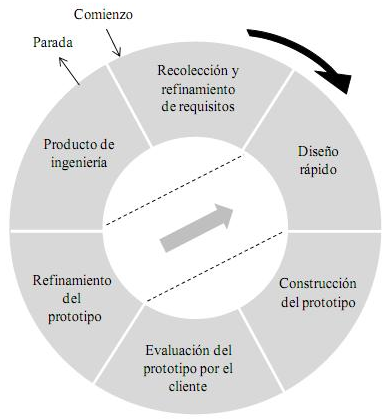
\includegraphics[width=0.5\textwidth]{img/chapter04/prototipo.png}
	\caption[Etapas de la metodología por prototipos.]{tapas de la metodología por prototipos. \textit{Fuente: ~\cite{MetodologíasDeDesarrollo2015}}}
	\label{fig:prototpios-metodología}  % Etiqueta para la figura
\end{figure}

El uso de prototipos evolutivos permite abordar los requerimientos del sistema de manera iterativa. Cada prototipo no es desechado sino que se refina progresivamente hasta obtener una versión completa del sistema. Esto asegura que el producto final no solo cumpla con los requisitos establecidos inicialmente, sino también con las expectativas del cliente o usuario. \newline \newline
La retroalimentación temprana que se recibe desde las primeras etapas del proyecto es invaluable para identificar mejoras y posibles problemas antes de que se conviertan en obstáculos mayores. Esto permite un ahorro significativo de tiempo y recursos, ya que se pueden realizar correcciones antes de que los problemas se propaguen en el ciclo de desarrollo. \newline \newline
A continuación, se muestra una tabla comparativa de ventajas/desventajas de utilizar esta metodología.
\begin{longtable}{|m{6.5cm}|m{6.5cm}|}
	\hline
	\rowcolor{black!75} \color{white}\textbf{Ventajas} & \color{white}\textbf{Desventajas} \\
	\hline
	Permite obtener retroalimentación temprana y frecuente del cliente, lo que ayuda a ajustar los requerimientos de manera rápida. &
	Puede generar una dependencia excesiva de los prototipos, llevando a malentendidos sobre la funcionalidad final del producto. \\
	\hline
	Facilita la detección temprana de errores o problemas de diseño, lo que reduce costos de desarrollo en fases posteriores. &
	Requiere recursos adicionales (tiempo y esfuerzo) para desarrollar y revisar los prototipos. \\
	\hline
	Mejora la comprensión de los requisitos por parte del equipo de desarrollo y el cliente, reduciendo malentendidos. &
	Si no se maneja adecuadamente, puede desviar el proyecto del alcance original, añadiendo características no planificadas (creeping scope). \\
	\hline
	Aumenta la satisfacción del cliente al ver un producto tangible en las primeras fases del desarrollo. &
	El prototipo puede ser confundido con el producto final, lo que puede generar expectativas irreales respecto a tiempos y calidad. \\
	\hline
	Fomenta la iteración y mejora continua del producto, asegurando que se ajuste mejor a las necesidades reales del cliente. &
	El uso excesivo de prototipos puede ralentizar el desarrollo del producto final si las iteraciones no están bien gestionadas. \\
	
	\hline
	\rowcolor{white} \caption{Ventajas/Desventajas de la metodología de Prototipos Evolutivos} \label{tabla:Ventajas-Desventajas-Prototipos} \\
\end{longtable}

\section{Análisis de Requerimientos}
El análisis de requerimientos tiene la finalidad de establecer las bases del proyecto, ya que permiten conocer si realmente se está entendiendo la problemática principal que se está tratando para garantizar que la solución propuesta es ideal para dar una solución fiable. 
Con esto en mente, partimos de los resultados de la encuesta y la investigación realizada en el estado del arte \ref{ch:Estado del Arte}, se han considerado los requerimientos que se detallan a continuación.
\subsection{Requerimientos Funcionales}
Los requerimientos funcionales describen lo que el sistema debe hacer, es decir, las funcionalidades o tareas específicas que debe realizar para cumplir su propósito. A continuación, se muestran en las siguientes tablas los requerimientos funcionales para el desarrollo del sistema cuyo proposito es calcular y graficar series de Fourier.

% Requerimiento 1
\begin{longtable}{|m{3.5cm}|m{9.5cm}|}
	\hline
	\rowcolor{black!75} \color{white}\textbf{Requerimiento} & \color{white}\textbf{Entrada para la función $f$} \\
	\hline
	\endfirsthead
	\multicolumn{2}{c}{{\tablename\ \thetable{} -- continuación}} \\
	\hline
	\rowcolor{black!75} \color{white}\textbf{Requerimiento} & \color{white}\textbf{Entrada para la función $f$} \\
	\hline
	\endhead
	\hline \multicolumn{2}{r}{{Continúa en la siguiente página}} \\
	\endfoot
	\hline
	\endlastfoot
	
	\textbf{Identificador} & RF1 \\
	\hline
	\textbf{Prioridad de desarrollo} & Alta \\
	\hline
	\textbf{Entrada} & Función \( f \) ingresada por el usuario, ya sea en términos de $x$ o de $t$, en formato de notación matemática, como una sola función o como una función a trozos incluyendo los intervalos de \(t\) o $x$. \\
	\hline
	\textbf{Salida} & Captura y representación de la función ingresada en notación matemática en la interfaz. \\
	\hline
	\textbf{Descripción} & El sistema permitirá al usuario ingresar una función \( f \), en un campo de entrada fácil de entender. Proporcionar botones de añadir (\scalebox{0.8}{\faIcon{plus-circle}}) y quitar (\scalebox{0.8}{\faIcon{minus-circle}}) para agregar o eliminar trozos de la función sin necesidad de preguntar explícitamente si es una función a trozos. \\
	\hline
	\textbf{Precondición} & El usuario debe estar en la interfaz de entrada de función. \\
	\hline
	\textbf{Postcondición} & La función ingresada se mostrará en notación matemática y estará lista para validación y procesamiento. \\
	\hline
\end{longtable}
\caption{Requerimiento funcional No. 1} \label{tabla:RF1}
\vspace{0.5cm}

% Requerimiento 2
\begin{longtable}{|m{3.5cm}|m{9.5cm}|}
	\hline
	\rowcolor{black!75} \color{white}\textbf{Requerimiento} & \color{white}\textbf{Teclado con fin} \\
	\hline
	\endfirsthead
	\multicolumn{2}{c}{{\tablename\ \thetable{} -- continuación}} \\
	\hline
	\rowcolor{black!75} \color{white}\textbf{Requerimiento} & \color{white}\textbf{Teclado con fin} \\
	\hline
	\endhead
	\hline \multicolumn{2}{r}{{Continúa en la siguiente página}} \\
	\endfoot
	\hline
	\endlastfoot
	
	\textbf{Identificador} & RF2 \\
	\hline
	\textbf{Prioridad de desarrollo} & Media \\
	\hline
	\textbf{Entrada} & Interacción del usuario con el teclado en pantalla para ingresar funciones y símbolos matemáticos como $sin()$, $cos()$, $sinh()$, $cosh()$, $exp()$, exponentes y fracciones. \\
	\hline
	\textbf{Salida} & Función correctamente ingresada en notación matemática en la interfaz de usuario, utilizando los símbolos seleccionados del teclado en pantalla. \\
	\hline
	\textbf{Descripción} & La interfaz debe mostrar un teclado en pantalla que incluya funciones matemáticas y símbolos comunes, tales como funciones trigonométricas ($sin()$, $cos()$), hiperbólicas ($cos()$, $sinh()$), exponenciales ($exp()$), operaciones de potencia y fracciones. Esto permitirá al usuario ingresar funciones de manera precisa y eficiente. \\
	\hline
	\textbf{Precondición} & El usuario debe tener acceso a la interfaz de entrada de funciones con el teclado en pantalla activado. \\
	\hline
	\textbf{Postcondición} & La función ingresada aparece en el campo de entrada en notación matemática, lista para su procesamiento. \\
	\hline
\end{longtable}
\captionof{table}{Requerimiento funcional No. 2} \label{tabla:RF2}
\vspace{0.5cm}

% Requerimiento 3
\begin{longtable}{|m{3.5cm}|m{9.5cm}|}
	\hline
	\rowcolor{black!75} \color{white}\textbf{Requerimiento} & \color{white}\textbf{tipo de función} \\
	\hline
	\endfirsthead
	\multicolumn{2}{c}{{\tablename\ \thetable{} -- continuación}} \\
	\hline
	\rowcolor{black!75} \color{white}\textbf{Requerimiento} & \color{white}\textbf{tipo de función} \\
	\hline
	\endhead
	\hline \multicolumn{2}{r}{{Continúa en la siguiente página}} \\
	\endfoot
	\hline
	\endlastfoot
	
	\textbf{Identificador} & RF3 \\
	\hline
	\textbf{Prioridad de desarrollo} & Media \\
	\hline
	\textbf{Entrada} & El usuario selecciona el tipo de serie a utilizar entre opciones de serie trigonométrica o serie exponencial compleja. Si selecciona la serie trigonométrica, puede optar por extensiones periódicas de rango completo o de medio rango (extensión par usando serie de cosenos o extensión impar usando serie de senos). \\
	\hline
	\textbf{Salida} & El tipo de serie y extensión seleccionados quedan registrados y configurados en la interfaz, listos para el cálculo de la serie correspondiente. \\
	\hline
	\textbf{Descripción} & El sistema permite al usuario seleccionar entre opciones de series de Fourier: serie trigonométrica o serie exponencial compleja. Para la serie trigonométrica, el usuario puede elegir entre una extensión periódica de rango completo (opción por defecto) o una extensión de medio rango (par o impar), con la condición de que la función comience en \( t = 0 \) para las extensiones de medio rango. Si para estas no se selecciona una extensión impar o par, automáticamente se tomará la extensión periódica que incluye senos y cosenos. \\
	\hline
	\textbf{Precondición} & El usuario debe estar en la interfaz de selección de series de Fourier y tener una función cargada para análisis de serie. \\
	\hline
	\textbf{Postcondición} & El tipo de serie y la extensión seleccionada quedan configurados y visibles en la interfaz para su validación y procesamiento. \\
	\hline
\end{longtable}
\caption{Requerimiento funcional No. 3} \label{tabla:RF3}
\vspace{0.5cm}

% Requerimiento 4
\begin{longtable}{|m{3.5cm}|m{9.5cm}|}
	\hline
	\rowcolor{black!75} \color{white}\textbf{Requerimiento} & \color{white}\textbf{Catálogo} \\
	\hline
	\endfirsthead
	\multicolumn{2}{c}{{\tablename\ \thetable{} -- continuación}} \\
	\hline
	\rowcolor{black!75} \color{white}\textbf{Requerimiento} & \color{white}\textbf{Catálogo} \\
	\hline
	\endhead
	\hline \multicolumn{2}{r}{{Continúa en la siguiente página}} \\
	\endfoot
	\hline
	\endlastfoot
	
	\textbf{Identificador} & RF4 \\
	\hline
	\textbf{Prioridad de desarrollo} & Alta \\
	\hline
	\textbf{Entrada} & Función ingresada por el usuario en el campo de entrada de funciones. \\
	\hline
	\textbf{Salida} & Mensaje de notificación en la interfaz si la función ingresada es inválida para el cálculo de la Serie de Fourier. \\
	\hline
	\textbf{Descripción} & El sistema debe contar con un catálogo de funciones no válidas para el cálculo de Series de Fourier, (como \( \ln(t) \), $csc(t)$). Si el usuario ingresa una función inválida, el sistema debe informarle y evitar el proceso de cálculo, asegurando que solo funciones compatibles continúen al procesamiento. \\
	\hline
	\textbf{Precondición} & El usuario ha ingresado una función para la validación previa al cálculo de la Serie de Fourier. \\
	\hline
	\textbf{Postcondición} & La función es verificada y, en caso de ser inválida, el sistema notifica al usuario y bloquea el cálculo de la Serie de Fourier para dicha función. \\
	\hline
\end{longtable}
\caption{Requerimiento funcional No. 4} \label{tabla:RF4}
\vspace{0.5cm}


% Requerimiento 5
\begin{longtable}{|m{3.5cm}|m{9.5cm}|}
	\hline
	\rowcolor{black!75} \color{white}\textbf{Requerimiento} & \color{white}\textbf{parseo ida} \\
	\hline
	\endfirsthead
	\multicolumn{2}{c}{{\tablename\ \thetable{} -- continuación}} \\
	\hline
	\rowcolor{black!75} \color{white}\textbf{Requerimiento} & \color{white}\textbf{parseo ida} \\
	\hline
	\endhead
	\hline \multicolumn{2}{r}{{Continúa en la siguiente página}} \\
	\endfoot
	\hline
	\endlastfoot
	
	\textbf{Identificador} & RF5 \\
	\hline
	\textbf{Prioridad de desarrollo} & Alta \\
	\hline
	\textbf{Entrada} & Expresión matemática ingresada por el usuario en formato de notación matemática (LaTeX). \\
	\hline
	\textbf{Salida} & Expresión convertida a un formato compatible para procesamiento matemático en el backend, enviada mediante una solicitud en formato JSON. \\
	\hline
	\textbf{Descripción} & El sistema debe interpretar y convertir las entradas matemáticas en notación LaTeX a un formato compatible con el motor de cálculo. Los datos convertidos se envían al backend a través de una solicitud para su procesamiento. \\
	\hline
	\textbf{Precondición} & El usuario ha ingresado una expresión matemática en la interfaz. \\
	\hline
	\textbf{Postcondición} & La expresión se encuentra en el backend en un formato adecuado para su procesamiento y evaluación matemática. \\
	\hline
\end{longtable}
\caption{Requerimiento funcional No. 5} \label{tabla:RF5}
\vspace{0.5cm}

% Requerimiento 6
\begin{longtable}{|m{3.5cm}|m{9.5cm}|}
	\hline
	\rowcolor{black!75} \color{white}\textbf{Requerimiento} & \color{white}\textbf{Nombre del requerimiento} \\
	\hline
	\endfirsthead
	\multicolumn{2}{c}{{\tablename\ \thetable{} -- continuación}} \\
	\hline
	\rowcolor{black!75} \color{white}\textbf{Requerimiento} & \color{white}\textbf{Nombre del requerimiento} \\
	\hline
	\endhead
	\hline \multicolumn{2}{r}{{Continúa en la siguiente página}} \\
	\endfoot
	\hline
	\endlastfoot
	
	\textbf{Identificador} & RF6 \\
	\hline
	\textbf{Prioridad de desarrollo} & Alta \\
	\hline
	\textbf{Entrada} & Función ingresada por el usuario y configuraciones para el cálculo de la Serie de Fourier, como el número de términos deseado en la expansión. \\
	\hline
	\textbf{Salida} & Serie de Fourier generada, con los coeficientes calculados \( a_0 \), \( a_n \), \( b_n \) o \( c_n \), y expansión de la serie hasta el número especificado de términos. \\
	\hline
	\textbf{Descripción} & El sistema utiliza un motor de cálculo simbólico en el backend para resolver los integrales necesarios, calcular los coeficientes de Fourier \( a_0 \), \( a_n \), \( b_n \) o \( c_n \), y generar la expansión de la Serie de Fourier hasta 50 términos. \\
	\hline
	\textbf{Precondición} & El usuario ha ingresado una función válida y configurado los parámetros para el cálculo de la Serie de Fourier. \\
	\hline
	\textbf{Postcondición} & La Serie de Fourier calculada y sus coeficientes se encuentran disponibles en la interfaz para visualización y análisis. \\
	\hline
\end{longtable}
\caption{Requerimiento funcional No. 6} \label{tabla:RF6}
\vspace{0.5cm}

% Requerimiento 7
\begin{longtable}{|m{3.5cm}|m{9.5cm}|}
	\hline
	\rowcolor{black!75} \color{white}\textbf{Requerimiento} & \color{white}\textbf{Nombre del requerimiento} \\
	\hline
	\endfirsthead
	\multicolumn{2}{c}{{\tablename\ \thetable{} -- continuación}} \\
	\hline
	\rowcolor{black!75} \color{white}\textbf{Requerimiento} & \color{white}\textbf{Nombre del requerimiento} \\
	\hline
	\endhead
	\hline \multicolumn{2}{r}{{Continúa en la siguiente página}} \\
	\endfoot
	\hline
	\endlastfoot
	
	\textbf{Identificador} & RF7 \\
	\hline
	\textbf{Prioridad de desarrollo} & Media \\
	\hline
	\textbf{Entrada} & Solicitud de recuperación de resultados generados por el cálculo de la Serie de Fourier, en formato JSON. \\
	\hline
	\textbf{Salida} & Resultados del cálculo, convertidos para visualización gráfica y en formato LaTeX para mostrar expresiones matemáticas en la interfaz. \\
	\hline
	\textbf{Descripción} & El sistema enviará los resultados del cálculo al frontend a través de una solicitud en formato JSON. La interfaz de usuario debe interpretar estos resultados y convertirlos a un formato adecuado para graficación y a formato LaTeX para mostrar las expresiones matemáticas en notación visual. \\
	\hline
	\textbf{Precondición} & Los resultados de los cálculos de la Serie de Fourier están listos para su recuperación y visualización en el frontend. \\
	\hline
	\textbf{Postcondición} & Los resultados se muestran en la interfaz de usuario en formato gráfico y en notación matemática (LaTeX) para una interpretación visual y análisis claros. \\
	\hline
\end{longtable}
\caption{Requerimiento funcional No. 7} \label{tabla:RF7}
\vspace{0.5cm}

% Requerimiento 8
\begin{longtable}{|m{3.5cm}|m{9.5cm}|}
	\hline
	\rowcolor{black!75} \color{white}\textbf{Requerimiento} & \color{white}\textbf{gráficas} \\
	\hline
	\endfirsthead
	\multicolumn{2}{c}{{\tablename\ \thetable{} -- continuación}} \\
	\hline
	\rowcolor{black!75} \color{white}\textbf{Requerimiento} & \color{white}\textbf{gráficas} \\
	\hline
	\endhead
	\hline \multicolumn{2}{r}{{Continúa en la siguiente página}} \\
	\endfoot
	\hline
	\endlastfoot
	
	\textbf{Identificador} & RF8 \\
	\hline
	\textbf{Prioridad de desarrollo} & Alta \\
	\hline
	\textbf{Entrada} & La función original \( f \) y su aproximación de Serie de Fourier, así como el número de términos especificado por el usuario. \\
	\hline
	\textbf{Salida} & Gráfica interactiva en la interfaz que muestra tanto la función original como su aproximación mediante Serie de Fourier. \\
	\hline
	\textbf{Descripción} & El sistema debe graficar la función original \( f \) y su aproximación mediante la Serie de Fourier en una interfaz gráfica interactiva. El usuario podrá ajustar el número de términos de la serie mediante un control deslizante, y contará con herramientas para hacer zoom, panear e interactuar en tiempo real con la gráfica. La representación gráfica debe ser eficiente y de alto rendimiento para asegurar una experiencia de usuario fluida. \\
	\hline
	\textbf{Precondición} & El usuario ha ingresado la función y solicitado la visualización gráfica de su aproximación mediante Serie de Fourier. \\
	\hline
	\textbf{Postcondición} & La gráfica interactiva de la función y su aproximación de Fourier se encuentra visible y responde a las interacciones del usuario. \\
	\hline
\end{longtable}
\caption{Requerimiento funcional No. 8} \label{tabla:RF8}
\vspace{0.5cm}

% Requerimiento 9
\begin{longtable}{|m{3.5cm}|m{9.5cm}|}
	\hline
	\rowcolor{black!75} \color{white}\textbf{Requerimiento} & \color{white}\textbf{resultados} \\
	\hline
	\endfirsthead
	\multicolumn{2}{c}{{\tablename\ \thetable{} -- continuación}} \\
	\hline
	\rowcolor{black!75} \color{white}\textbf{Requerimiento} & \color{white}\textbf{resultados} \\
	\hline
	\endhead
	\hline \multicolumn{2}{r}{{Continúa en la siguiente página}} \\
	\endfoot
	\hline
	\endlastfoot
	
	\textbf{Identificador} & RF9 \\
	\hline
	\textbf{Prioridad de desarrollo} & Media \\
	\hline
	\textbf{Entrada} & Coeficientes calculados \( a_0 \), \( a_n \), \( b_n \), \( c_n \), y la expresión completa de la Serie de Fourier para la función \( f(t) \). \\
	\hline
	\textbf{Salida} & Visualización clara y legible de los coeficientes calculados, la función original \( f(t) \), y la expansión de la Serie de Fourier. \\
	\hline
	\textbf{Descripción} & El sistema debe mostrar los coeficientes \( a_0 \), \( a_n \), \( b_n \) y \( c_n \), junto con la función original \( f \) y su expansión en Series de Fourier $f = \sum$. Las expresiones matemáticas deben presentarse de manera clara y legible, permitiendo al usuario comprender y revisar los cálculos y resultados de forma efectiva. \\
	\hline
	\textbf{Precondición} & Los coeficientes de la Serie de Fourier y la expansión han sido calculados y están listos para su visualización. \\
	\hline
	\textbf{Postcondición} & Las expresiones matemáticas se muestran de manera clara en la interfaz, facilitando la interpretación y revisión de los resultados por parte del usuario. \\
	\hline
\end{longtable}
\caption{Requerimiento funcional No. 9} \label{tabla:RF9}
\vspace{0.5cm}

% Requerimiento 10
\begin{longtable}{|m{3.5cm}|m{9.5cm}|}
	\hline
	\rowcolor{black!75} \color{white}\textbf{Requerimiento} & \color{white}\textbf{Nombre del requerimiento} \\
	\hline
	\endfirsthead
	\multicolumn{2}{c}{{\tablename\ \thetable{} -- continuación}} \\
	\hline
	\rowcolor{black!75} \color{white}\textbf{Requerimiento} & \color{white}\textbf{Nombre del requerimiento} \\
	\hline
	\endhead
	\hline \multicolumn{2}{r}{{Continúa en la siguiente página}} \\
	\endfoot
	\hline
	\endlastfoot
	
	\textbf{Identificador} & RF10 \\
	\hline
	\textbf{Prioridad de desarrollo} & Media \\
	\hline
	\textbf{Entrada} & Interacciones del usuario, como el ingreso de valores en el sistema o ajustes en el número de términos de la Serie de Fourier. \\
	\hline
	\textbf{Salida} & Mensajes de error claros en caso de entradas no válidas o errores de cálculo, y retroalimentación visual inmediata en la interfaz cuando se ajusta el número de términos o se interactúa con la gráfica. \\
	\hline
	\textbf{Descripción} & El sistema debe ofrecer mensajes de error informativos cuando el usuario ingrese datos no válidos o se produzcan errores de cálculo, mejorando la comprensión del usuario sobre la naturaleza del problema.\\
	\hline
	\textbf{Precondición} & El usuario está interactuando con la interfaz de la Serie de Fourier, ya sea ingresando valores o manipulando la gráfica. \\
	\hline
	\textbf{Postcondición} & El usuario recibe mensajes de error informativos y retroalimentación visual en tiempo real, lo cual facilita una interacción más eficiente y comprensible con el sistema. \\
	\hline
\end{longtable}
\caption{Requerimiento funcional No. 10} \label{tabla:RF10}
\vspace{0.5cm}




\subsection{Requerimientos No Funcionales}
Los requerimientos funcionales definen cómo debe funcionar el sistema, estableciendo estándares de calidad como rendimiento, seguridad, usabilidad, escalabilidad, y eficiencia.

%Tabla de no funcionales
\begin{longtable}{|m{5cm}|m{10cm}|}
	\hline
	\rowcolor{black!75} \color{white}\textbf{Nombre} & \color{white}\textbf{Descripción} \\
	\hline
	\rowcolor{black!75}
	\head {Nombre} & \head {Descripción} \\ \hline
	\endfirsthead
	\multicolumn{2}{c}{{\tablename\ \thetable{} -- continuación}} \\
	\rowcolor{black!75}
	\head {Nombre} & \head {Descripción}\\ \hline
	\endhead
	\hline \multicolumn{2}{r}{{Continúa en la siguiente página}} \\
	\endfoot
	\hline
	\endlastfoot
	\textbf{Rendimiento y Escalabilidad} & El sistema debe calcular los coeficientes de Fourier en un tiempo razonable, incluso para funciones con múltiples trozos o con un alto número de términos en la serie. La visualización gráfica debe ser fluida y responsiva, incluso al agregar o quitar muchos términos de la serie. Las interacciones en el lienzo canvas deben realizarse sin latencia perceptible. \\
	\hline
	\textbf{Interfaz de Usuario Amigable e Intuitiva} & La interfaz debe ser intuitiva y fácil de usar, con botones y controles claramente identificados. Los mensajes de error y advertencia deben ser comprensibles, evitando el uso de jerga técnica complicada. La notación matemática debe ser clara y precisa, usando MathQuill para entradas y visualización de resultados. \\
	\hline
	\textbf{Manejo de la Concurrencia} & La aplicación debe soportar múltiples usuarios concurrentes enviando cálculos al backend sin generar bloqueos ni conflictos en las llamadas a Maxima. \\
	\hline
	\textbf{Portabilidad y Compatibilidad} & La aplicación debe ser compatible con los principales navegadores modernos (Chrome, Firefox, Edge). Aunque no es recomendable usar la aplicación en dispositivos móviles, el diseño debe ser responsivo para ajustarse a diferentes tamaños de pantalla, incluidos dispositivos móviles y tabletas. \\
	\hline
	\textbf{Modularidad y Extensibilidad del Código} & El frontend debe estar diseñado para facilitar la migración a frameworks como Angular en el futuro. El código debe ser modular y seguir buenas prácticas de desarrollo para facilitar la adición de nuevas características. Aunque el sistema no requiere una base de datos en su versión actual, el backend debe ser fácilmente extensible para permitir el almacenamiento de sesiones o configuraciones del usuario en el futuro. \\
	\hline
	\textbf{Seguridad de la Aplicación} & Las peticiones a la API deben estar protegidas contra inyecciones de código. Implementar seguridad básica en el backend para evitar solicitudes maliciosas o repetitivas que puedan afectar el rendimiento del servicio. \\
	\hline
	\textbf{Mantenibilidad de Código} & La aplicación debe tener una guía de usuario clara para explicar cómo ingresar funciones, seleccionar series y usar la interfaz. El código debe estar bien documentado para que futuros desarrolladores puedan entender la lógica y estructura de la aplicación fácilmente. \\
	\hline
%	\textbf{Tiempo de Respuesta del Sistema} & El tiempo de respuesta del servidor para calcular coeficientes de Fourier no debe exceder los 5 segundos en condiciones normales. La gráfica debe actualizarse en menos de 500 ms para proporcionar una experiencia interactiva y sin latencia. \\
%	\hline
%	\textbf{Consumo de Recursos} & La aplicación debe ser eficiente en el uso de memoria y CPU, especialmente al realizar cálculos de series grandes. El uso de canvas debe estar optimizado para no causar retrasos en la interfaz. \\
%	\hline
%	\textbf{Compatibilidad con Carga Asíncrona} & La comunicación entre el frontend y el backend debe ser asíncrona para no bloquear la interfaz de usuario. Las llamadas a Maxima deben ser gestionadas de manera eficiente para evitar cuellos de botella. \\
%	\hline
	%\rowcolor{white} \caption{Tabla de requerimientos no funcionales} \label{tabla:RNF} \\
\end{longtable}
\caption{Tabla de requerimientos no funcionales} \label{tabla:RNF}
\vspace{0.5cm}



\section{Análisis de Riesgos}
En la gestión de proyectos, los riesgos representan cualquier evento o condición incierta que, si ocurre, puede afectar negativamente los objetivos del proyecto. Identificar y gestionar estos riesgos es crucial para minimizar su impacto y asegurar el éxito del proyecto. 
\subsection{Matriz de riesgos}
La matriz de riesgos es una herramienta clave en la gestión de proyectos, ya que permite evaluar y visualizar la gravedad y probabilidad de los riesgos que pueden afectar su éxito. Clasifica los riesgos según sus consecuencias (de "bajo" a "grave") y su frecuencia de ocurrencia (de "raro" a "casi seguro"). Al organizar estos factores en una matriz de cinco por cinco, es más fácil identificar los riesgos más críticos y priorizar las acciones correctivas. Los colores de la matriz van del verde (bajo riesgo) al rojo (alto riesgo), lo que proporciona una representación visual clara de la urgencia y el impacto de cada riesgo identificado \ref{tabla:matriz_riesgos}.

\begin{table}[H]
	\centering
	\begin{tabular}{|>{\centering\arraybackslash}m{4cm}|c|c|c|c|c|}
		\hline
		\rowcolor{black!75} \color{white} {\textbf{Consecuencias}} & \multicolumn{5}{c|}{ \color{white} \textbf{Probabilidad}} \\ \cline{2-6}
		\cellcolor{white} & \textbf{Casi seguro} & \textbf{Probable} & \textbf{Posible} & \textbf{Improbable} & \textbf{Raro} \\ \hline
		\textbf{Grave} & \cellcolor{red!80}Extremo & \cellcolor{red!80}Extremo & \cellcolor{red!80}Extremo & \cellcolor{orange!80}Alto & \cellcolor{yellow!60}Medio \\ \hline
		\textbf{Mayor} & \cellcolor{red!80}Extremo & \cellcolor{red!80}Extremo & \cellcolor{orange!80}Alto & \cellcolor{yellow!60}Medio & \cellcolor{yellow!60}Medio \\ \hline
		\textbf{Moderado} & \cellcolor{red!80}Extremo & \cellcolor{orange!80}Alto & \cellcolor{yellow!60}Medio & \cellcolor{yellow!60}Medio & \cellcolor{green!60}Bajo \\ \hline
		\textbf{Menor} & \cellcolor{orange!80}Alto & \cellcolor{yellow!60}Medio & \cellcolor{yellow!60}Medio & \cellcolor{green!60}Bajo & \cellcolor{green!60}Bajo \\ \hline
		\textbf{Bajo} & \cellcolor{yellow!60}Medio & \cellcolor{yellow!60}Medio & \cellcolor{green!60}Bajo & \cellcolor{green!60}Bajo & \cellcolor{green!60}Bajo \\ \hline
	\end{tabular}
	\caption[Matriz de clasificación de riesgos.]{Matriz de clasificación de riesgos. \textit{Fuente: Elaboración propia}}
	\label{tabla:matriz_riesgos}
\end{table}


\subsection{Identificación y jerarquización de riesgos}
Para poder comenzar con el análisis de riesgos pertinente, comenzamos identificación los riesgos que pueden ocurrir y, por lo tanto, afectar la correcta ejecución del proyecto, además de su jerarquización en base a su semáforo.


\begin{longtable}{|m{1.5cm}|m{5.3cm}|m{3cm}|m{2cm}|m{2cm}|}
	\rowcolor{black!75} \color{white} \textbf{ID Riesgo} & \color{white} \textbf{Descripción} & \color{white} \textbf{Probabilidad} & \color{white} \textbf{Impacto} & \color{white} \textbf{Semáforo} \\ \hline
	\textbf{R1} & Incapacidad temporal para continuar el proyecto debido a una enfermedad u otra causa que afecte la salud o disponibilidad. & Posible & Grave & \cellcolor{red!80} \\ \hline
	\textbf{R2} & Mala gestión del tiempo y actividades a  lo largo del desarrollo del proyecto. & Posible & Mayor & \cellcolor{orange!80} \\ \hline
	\textbf{R3} & Mala elección de tecnologías para el desarrollo del proyecto & Posible & Mayor & \cellcolor{orange!80} \\ \hline
	\textbf{R4} & Falta de claridad o mal planteamiento de los requerimientos & Posible & Mayor & \cellcolor{orange!80} \\ \hline
	\textbf{R5} & No cumplir con los objetivos del proyecto & Posible & Mayor & \cellcolor{red!80} \\ \hline
	\textbf{R6} & Falta de conocimientos para realizar actividades relacionadas al proyecto. & Medio & Grave &  \cellcolor{yellow!60} \\ \hline
	\textbf{R6} & Sobrecarga de y proyectos académicos & Probable & Mayor &  \cellcolor{red!80}  \\ \hline
	\textbf{R7} & Sobrecarga de y proyectos académicos & Probable & Mayor &  \cellcolor{red!80}  \\ \hline
	\rowcolor{white} \caption{Tabla de identificación de riesgos} \label{tabla:riesgos} \\
	
\end{longtable}

\subsection{Jerarquización de Riesgos}

\section{Estimación de Costos}
\subsection{Método de Estimación de Costos}
\subsection{Detalle de los Costos Estimados}

\section{Diseño del Sistema}
\subsection{Arquitectura General del Sistema}
\subsubsection{Arquitectura Cliente-Servidor}
\subsubsection{Flujo de Datos}

\subsection{Diseño de la Interfaz de Usuario}
\subsubsection{Estructura de la Interfaz}
\subsubsection{Prototipo de la Interfaz}
